\chapter{Bosons composites, représentations du spin et doublement de Dirac}

\section{Symétrie d’échange et bosons composites}

La question initiale constitue un véritable paradoxe concernant les particules composites. Si deux fermions forment un boson, deux bosons de ce type peuvent-ils occuper le même état sans enfreindre le principe d’exclusion des fermions ? La réponse part de la règle d’échange elle-même.

Supposons que deux particules identiques soient décrites par une fonction d’onde à deux arguments. Les symboles \(x\) et \(y\) désignent les deux emplacements des particules ; ils ne distinguent pas deux espèces. La fonction d’onde est symétrique pour les bosons et antisymétrique pour les fermions :
\begin{equation}
\Psi_B(x,y)=\Psi_B(y,x),
\qquad
\Psi_F(x,y)=-\Psi_F(y,x).
\end{equation}
Cette symétrie signifie que l’échange des deux particules indiscernables ne produit pas un nouvel état physique.

Deux bosons peuvent tout à fait occuper le même état à une particule. Si cet état a pour fonction d’onde \(\varphi\), le produit à deux particules est
\begin{equation}
\Psi(x,y)=\varphi(x)\varphi(y).
\end{equation}
Les fonctions d’onde sont des fonctions ordinaires à valeurs complexes, et non des opérateurs ou des matrices ; leurs valeurs commutent donc :
\begin{equation}
\varphi(x)\varphi(y)=\varphi(y)\varphi(x).
\end{equation}
Le produit est donc symétrique. La même construction ne peut pas donner un état non nul de deux fermions, car l’antisymétrie imposerait
\begin{equation}
\varphi(x)\varphi(y)=-\varphi(y)\varphi(x),
\end{equation}
alors que les deux membres sans le signe moins sont égaux.

Plus généralement, partons d’une fonction d’onde à deux particules quelconque \(F(x,y)\), sans supposer qu’elle possède une symétrie d’échange. Ses parties symétrique et antisymétrique sont, à un facteur de normalisation près,
\begin{align}
F_{\mathrm{sym}}(x,y)&=F(x,y)+F(y,x),\\
F_{\mathrm{asym}}(x,y)&=F(x,y)-F(y,x).
\end{align}
La vérification de l’échange est explicite :
\begin{align}
F_{\mathrm{sym}}(y,x)
&=F(y,x)+F(x,y)
=F_{\mathrm{sym}}(x,y),\\
F_{\mathrm{asym}}(y,x)
&=F(y,x)-F(x,y)
=-F_{\mathrm{asym}}(x,y).
\end{align}
Ajouter la fonction échangée rend la fonction symétrique ; la soustraire la rend antisymétrique.

Une paire d’atomes d’hydrogène offre un cas plus intéressant. Elle comporte quatre fermions constitutifs : deux électrons identiques et deux protons identiques. Désignons par \(x_1,x_2\) les variables des électrons et par \(y_1,y_2\) celles des protons. La fonction d’onde à quatre corps doit être antisymétrique séparément sous l’échange des électrons et sous celui des protons :
\begin{align}
\Psi(x_2,x_1;y_1,y_2)
&=-\Psi(x_1,x_2;y_1,y_2),\\
\Psi(x_1,x_2;y_2,y_1)
&=-\Psi(x_1,x_2;y_1,y_2).
\end{align}

Pour motiver l’introduction de deux fonctions d’onde distinctes pour un atome, imaginons un atome d’hydrogène localisé près de l’origine, de fonction d’onde \(\psi(x,y)\), et un autre localisé ailleurs, de fonction d’onde \(\phi(x,y)\). La seconde peut simplement être une copie de la première translatée, obtenue en translatant les arguments de son électron et de son proton, mais elle reste une fonction d’onde distincte dans cette configuration. Un produit naïf est
\begin{equation}
\psi(x_1,y_1)\phi(x_2,y_2).
\end{equation}
Il ne possède encore aucune des deux antisymétries fermioniques requises.

Commençons par antisymétriser les variables des électrons :
\begin{equation}
\Psi_x=
\psi(x_1,y_1)\phi(x_2,y_2)
-\psi(x_2,y_1)\phi(x_1,y_2).
\end{equation}
Sous \(x_1\leftrightarrow x_2\), les deux termes s’échangent et l’expression entière change de signe. Antisymétrisons maintenant ce résultat par rapport aux variables des protons. L’ordre des quatre termes est déterminé par ces deux antisymétrisations successives.\footnote{Cette construction fixe également la suite de signes \(+,-,-,+\), après correction des étiquettes de variables dans le calcul oral.}
\begin{align}
\Psi_{2H}(x_1,x_2;y_1,y_2)
&=\Psi_x(x_1,x_2;y_1,y_2)\nonumber\\
&\quad{}-\Psi_x(x_1,x_2;y_2,y_1)\\
&=\psi(x_1,y_1)\phi(x_2,y_2)\nonumber\\
&\quad{}-\psi(x_2,y_1)\phi(x_1,y_2)\nonumber\\
&\quad{}-\psi(x_1,y_2)\phi(x_2,y_1)\nonumber\\
&\quad{}+\psi(x_2,y_2)\phi(x_1,y_1).
\label{eq:two-hydrogen-antisymmetrized}
\end{align}
L’échange des électrons permute les deux premiers termes ainsi que les deux derniers, et inverse le signe de l’expression entière. Il en va de même pour l’échange des protons. L’état possède donc exactement les deux antisymétries distinctes requises pour les fermions constitutifs.

\begin{classroomqa}\lecturetimestamp{00:11:11}\audiencequestion{Si les atomes d’hydrogène sont des bosons, qu’est-ce qui empêche d’en placer deux exactement l’un sur l’autre ?}\lecturerresponse{Les statistiques d’échange bosoniques ne suppriment pas les forces entre les atomes. Le principe d’exclusion de Pauli appliqué aux constituants, ainsi que les autres forces interatomiques, peut rendre le recouvrement spatial extrêmement coûteux en énergie. C’est une question différente de celle de savoir si les atomes peuvent occuper le même état de quantité de mouvement délocalisé. Un état propre de l’impulsion est étendu dans tout l’espace ; avoir la même impulsion ne signifie donc pas que les atomes sont projetés au même point. Même des objets à cœur dur, comme des boules de billard, pourraient obéir aux statistiques d’échange bosoniques : leur cœur dur empêcherait le recouvrement spatial, tandis que les statistiques bosoniques permettraient toujours une occupation commune en impulsion.}\end{classroomqa}

\begin{classroomqa}\lecturetimestamp{00:12:28}\audiencequestion{Placer deux atomes d’hydrogène dans le même état propre de l’impulsion placerait-il leurs fermions constitutifs dans le même état ?}\lecturerresponse{Non. L’état à quatre corps reste antisymétrique sous l’échange des deux variables électroniques, et séparément antisymétrique sous celui des deux variables protoniques. Seul l’échange simultané des deux constituants---, c’est-à-dire l’échange des deux atomes entiers---, est symétrique.}\end{classroomqa}

En effet, échanger les deux atomes revient à effectuer les deux substitutions
\begin{equation}
x_1\leftrightarrow x_2,
\qquad
y_1\leftrightarrow y_2.
\end{equation}
La première substitution apporte un signe moins fermionique, et la seconde en apporte un autre :
\begin{equation}
\begin{aligned}
\Psi_{2H}(x_2,x_1;y_2,y_1)
&=(-1)(-1)\Psi_{2H}(x_1,x_2;y_1,y_2)\\
&=\Psi_{2H}(x_1,x_2;y_1,y_2).
\end{aligned}
\end{equation}
On peut obtenir le même résultat en examinant les termes un à un dans l’équation~\eqref{eq:two-hydrogen-antisymmetrized}. Lors de l’échange des atomes entiers,
\begin{equation}
\psi(x_1,y_1)\phi(x_2,y_2)
\longleftrightarrow
\psi(x_2,y_2)\phi(x_1,y_1),
\end{equation}
le premier et le quatrième termes s’échangent. De même,
\begin{equation}
-\psi(x_2,y_1)\phi(x_1,y_2)
\longleftrightarrow
-\psi(x_1,y_2)\phi(x_2,y_1),
\end{equation}
le deuxième et le troisième termes s’échangent. L’état complet est symétrique sous l’échange des atomes. Deux signes moins dus aux constituants donnent un signe plus pour le composite.

Cette propriété d’échange est logiquement indépendante de l’énergie nécessaire pour que les atomes se recouvrent. Une forte répulsion peut rendre un tel recouvrement inaccessible, mais elle ne modifie pas la loi d’échange symétrique.

\begin{classroomqa}\lecturetimestamp{00:14:42}\audiencequestion{Que représente physiquement l’état à quatre corps construit ici, et s’agit-il spécifiquement d’un état dans l’espace des impulsions ?}\lecturerresponse{C’est la fonction d’onde de deux atomes obtenue à partir de deux fonctions d’onde à un atome, en antisymétrisant d’abord les étiquettes des électrons, puis celles des protons. Il n’est pas nécessaire de l’écrire dans l’espace des impulsions. Les variables peuvent décrire la position, l’impulsion ou une autre représentation ; les symétries d’échange requises pour les constituants restent les mêmes.}\end{classroomqa}

Par conséquent, deux atomes peuvent occuper la même fonction d’onde d’impulsion délocalisée, même si contraindre leurs distributions spatiales à se recouvrir fortement peut coûter beaucoup d’énergie.

Posons maintenant les deux fonctions d’onde atomiques égales, \(\phi=\psi\). L’équation~\eqref{eq:two-hydrogen-antisymmetrized} devient
\begin{align}
\Psi_{\mathrm{same}}
&=\psi(x_1,y_1)\psi(x_2,y_2)
-\psi(x_2,y_1)\psi(x_1,y_2)\nonumber\\
&\quad
-\psi(x_1,y_2)\psi(x_2,y_1)
+\psi(x_2,y_2)\psi(x_1,y_1).
\end{align}

Cet état à quatre corps s’annule-t-il ? Non. Le premier et le quatrième produits sont égaux, de même que le deuxième et le troisième. En utilisant la commutativité des fonctions d’onde atomiques,
\begin{equation}
\Psi_{\mathrm{same}}
=
2\left[
\psi(x_1,y_1)\psi(x_2,y_2)
-\psi(x_2,y_1)\psi(x_1,y_2)
\right],
\label{eq:same-hydrogen-state}
\end{equation}
qui est généralement non nul. Il reste antisymétrique par rapport aux deux variables électroniques et séparément par rapport aux deux variables protoniques.

On n’attribue pas ici un électron nettement localisé à chaque atome nettement localisé. Un électron lié dans un atome est délocalisé dans l’espace sur l’étendue de la fonction d’onde atomique. Donner aux deux atomes le même état atomique ne pose donc ni \(x_1=x_2\), ni \(y_1=y_2\).

On peut constater directement l’exclusion des constituants en examinant la coïncidence. Si les deux arguments électroniques modélisés coïncident, \(x_1=x_2=x\), l’équation~\eqref{eq:same-hydrogen-state} donne
\begin{align}
\Psi_{\mathrm{same}}(x,x;y_1,y_2)
&=2\bigl[
\psi(x,y_1)\psi(x,y_2)\nonumber\\
&\quad{}-\psi(x,y_1)\psi(x,y_2)
\bigr]\\
&=0.
\end{align}
L’expression correspondante s’annule aussi lorsque \(y_1=y_2\). Ainsi, la fonction d’onde composite dans un même état est non nulle, tandis que son amplitude s’annule lorsque les arguments de fermions identiques coïncident.\footnote{Dans ce modèle, le spin et les autres étiquettes à une particule ne sont pas pris en compte. L’antisymétrie fermionique s’applique à l’ensemble des étiquettes d’une particule ; l’annulation présentée ici concerne la coïncidence des arguments conservés dans le modèle.}

\begin{classroomqa}\lecturetimestamp{00:20:41}\audiencequestion{Les atomes peuvent-ils être dans le même état alors que leurs électrons et leurs protons ne sont pas dans les mêmes états constitutifs ?}\lecturerresponse{Oui. L’égalité des fonctions d’onde atomiques composites ne supprime pas les antisymétries distinctes des électrons et des protons. L’état complet à quatre corps peut décrire deux atomes dans un seul et même état atomique tout en attribuant une amplitude nulle aux arguments de fermions identiques qui coïncident.}\end{classroomqa}

\begin{classroomqa}\lecturetimestamp{00:21:12}\audiencequestion{L’antisymétrisation a-t-elle éliminé les composantes où les constituants identiques coïncident ?}\lecturerresponse{Oui. Dans les variables présentées ici, ces composantes de coïncidence s’annulent exactement. Plus précisément, la fonction d’onde antisymétrique s’annule lorsque les arguments des deux fermions identiques sont égaux.}\end{classroomqa}

Cette annulation ne dépendait pas du fait d’avoir d’abord rendu égales les fonctions d’onde atomiques. Pour l’état général de l’équation~\eqref{eq:two-hydrogen-antisymmetrized},
\begin{align}
\Psi_{2H}(x,x;y_1,y_2)
&=\psi(x,y_1)\phi(x,y_2)\nonumber\\
&\quad{}-\psi(x,y_1)\phi(x,y_2)\nonumber\\
&\quad{}-\psi(x,y_2)\phi(x,y_1)\nonumber\\
&\quad{}+\psi(x,y_2)\phi(x,y_1)\\
&=0.
\end{align}

\begin{classroomqa}\lecturetimestamp{00:21:32}\audiencequestion{Cette annulation a-t-elle toujours lieu lorsque les atomes sont dans des états différents et que les variables de constituants identiques coïncident ?}\lecturerresponse{Oui. Elle découle de l’antisymétrie elle-même, et non du fait de poser \(\phi=\psi\). La même propriété vaut dans une autre représentation : après passage à l’espace des impulsions, l’amplitude s’annule lorsque les deux arguments d’impulsion des fermions identiques coïncident, pourvu que les autres étiquettes à une particule, omises ici, coïncident elles aussi.}\end{classroomqa}

\section{Le spin comme système quantique de dimension finie}

Les mathématiques du spin réapparaissent dans l’isospin, la couleur et les autres symétries internes de la physique des particules. L’analogie est formelle : la même algèbre intervient, même si les grandeurs physiques ne reçoivent pas nécessairement la même interprétation. L’objectif immédiat est d’approfondir un peu le spin, puis de revenir à l’équation de Dirac. Ces outils serviront ensuite à étudier l’isospin, concept associé historiquement aux années 1930.

L’électron est une particule de spin \(\tfrac12\), tout comme le proton et le muon. Sa composante de spin selon \(z\) peut prendre deux valeurs. Avant de fixer les unités, écrivons
\begin{equation}
S_z=m\hbar.
\end{equation}
Désormais, \(\hbar=1\). La lettre \(L\) est conventionnellement réservée au moment cinétique orbital ; le spin intrinsèque sera donc désigné par \(S\). Il obéit à la même algèbre du moment cinétique :
\begin{equation}
[S_x,S_y]=iS_z,
\quad
[S_y,S_z]=iS_x,
\quad
[S_z,S_x]=iS_y,
\end{equation}
et
\begin{equation}
S_\pm=S_x\pm iS_y.
\end{equation}
L’opérateur \(S_+\) augmente la valeur propre de \(S_z\) et \(S_-\) la diminue.

\begin{classroomqa}\lecturetimestamp{00:25:39}\audiencequestion{La discussion porte-t-elle spécifiquement sur le spin intrinsèque ?}\lecturerresponse{C’est bien le spin intrinsèque qui nous intéresse ici. La même algèbre du moment cinétique s’applique plus généralement, notamment au moment cinétique orbital ou à la rotation d’un objet macroscopique.}\end{classroomqa}

Pour le spin un demi, les seules valeurs propres de \(S_z\) sont \(+\tfrac12\) et \(-\tfrac12\). Pour l’instant, faisons abstraction de tout le reste concernant l’électron : oublions sa position et son impulsion et ne conservons que ses deux états de spin. Alors
\begin{equation}
|\psi\rangle
=
\alpha|\uparrow_z\rangle+\beta|\downarrow_z\rangle
\quad\longleftrightarrow\quad
\begin{pmatrix}
\alpha\\
\beta
\end{pmatrix},
\end{equation}
où
\begin{equation}
|\alpha|^2=P(\uparrow_z),
\qquad
|\beta|^2=P(\downarrow_z),
\qquad
|\alpha|^2+|\beta|^2=1.
\end{equation}
Il s’agit d’un espace d’états bidimensionnel. Cela ne signifie pas que l’espace ordinaire a deux dimensions.

\begin{classroomqa}\lecturetimestamp{00:28:18}\audiencequestion{A-t-on dit que l’espace physique était bidimensionnel ?}\lecturerresponse{Non. L’espace des états de spin est bidimensionnel. La position et l’impulsion ont été temporairement mises de côté, comme si l’électron était cloué à un mur et que seul son spin pouvait être mesuré.}\end{classroomqa}

Les opérateurs sur cet espace d’états sont représentés par des matrices \(2\times2\). Il est commode de choisir la base \(S_z\) de sorte que \(S_z\) soit diagonale, mais la diagonalité relève d’un choix de base et non d’une exigence physique.

\begin{classroomqa}\lecturetimestamp{00:29:46}\audiencequestion{Faut-il que \(S_z\) soit diagonale ?}\lecturerresponse{Non. On la choisit diagonale par commodité. D’autres représentations matricielles sont physiquement équivalentes.}\end{classroomqa}

\begin{classroomqa}\lecturetimestamp{00:30:08}\audiencequestion{\(S_z\) est-elle une matrice ?}\lecturerresponse{\(S_z\) est une observable, donc un opérateur. Dans la base de dimension finie choisie, cet opérateur est représenté par une matrice qui agit sur les vecteurs d’état.}\end{classroomqa}

Une représentation particulièrement utile est
\begin{equation}
S_i=\frac12\sigma_i,
\end{equation}
où
\begin{equation}
\sigma_x=
\begin{pmatrix}
0&1\\
1&0
\end{pmatrix},
\quad
\sigma_y=
\begin{pmatrix}
0&-i\\
i&0
\end{pmatrix},
\quad
\sigma_z=
\begin{pmatrix}
1&0\\
0&-1
\end{pmatrix}.
\end{equation}
Les matrices sans le facteur un demi sont les matrices de Pauli ; les opérateurs de spin eux-mêmes comportent ce facteur. Une multiplication directe vérifie les relations de commutation. Cette représentation n’est pas unique : une rotation des axes ou un changement de base donne un autre triplet équivalent.

Il s’agit d’une représentation à deux composantes du moment cinétique de spin un demi.

\subsection{États propres selon les axes de coordonnées}

Il est utile de résoudre les équations aux valeurs propres composante par composante. Comme les valeurs propres de \(\sigma_i\) sont \(\pm1\), celles de \(S_i=\sigma_i/2\) sont \(\pm\tfrac12\).

Pour \(\sigma_z\), les deux équations sont
\begin{align}
\begin{pmatrix}
1&0\\
0&-1
\end{pmatrix}
\begin{pmatrix}
\alpha\\
\beta
\end{pmatrix}
&=
\begin{pmatrix}
\alpha\\
\beta
\end{pmatrix},
&
\begin{pmatrix}
1&0\\
0&-1
\end{pmatrix}
\begin{pmatrix}
\alpha\\
\beta
\end{pmatrix}
&=
-
\begin{pmatrix}
\alpha\\
\beta
\end{pmatrix}.
\end{align}

\begin{figure}[t]
\centering
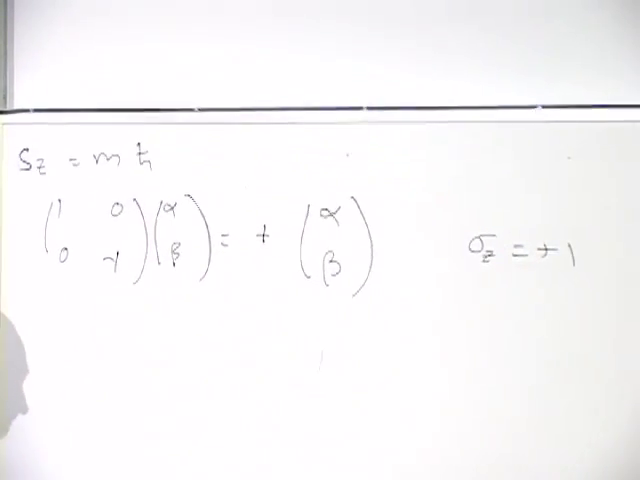
\includegraphics[width=0.74\textwidth]{lecture_08_figure_02.png}
\caption{Équation aux valeurs propres de \(+1\) pour \(\sigma_z\), agissant sur un spineur à deux composantes.}
\lectureframe{00:34:57}\end{figure}

Pour la valeur propre \(+1\), la multiplication ligne par ligne donne
\begin{equation}
\begin{pmatrix}
1\cdot\alpha+0\cdot\beta\\
0\cdot\alpha-\beta
\end{pmatrix}
=
\begin{pmatrix}
\alpha\\
-\beta
\end{pmatrix}
=
\begin{pmatrix}
\alpha\\
\beta
\end{pmatrix}.
\end{equation}
L’équation du haut est automatiquement satisfaite, tandis que celle du bas donne \(-\beta=\beta\), donc \(\beta=0\). La normalisation impose \(|\alpha|=1\) ; en choisissant la phase globale, sans conséquence physique, telle que \(\alpha=1\),
\begin{equation}
|+z\rangle=
\begin{pmatrix}
1\\
0
\end{pmatrix}.
\end{equation}

Pour la valeur propre \(-1\),
\begin{equation}
\begin{pmatrix}
\alpha\\
-\beta
\end{pmatrix}
=
\begin{pmatrix}
-\alpha\\
-\beta
\end{pmatrix}.
\end{equation}
Cette fois, l’équation du bas est automatiquement satisfaite et celle du haut donne \(\alpha=-\alpha\), donc \(\alpha=0\). En choisissant \(\beta=1\), on obtient
\begin{equation}
|-z\rangle=
\begin{pmatrix}
0\\
1
\end{pmatrix}.
\end{equation}

Changeons maintenant l’expérience et mesurons \(S_x\). Puisque
\begin{equation}
\sigma_x
\begin{pmatrix}
\alpha\\
\beta
\end{pmatrix}
=
\begin{pmatrix}
0\cdot\alpha+\beta\\
\alpha+0\cdot\beta
\end{pmatrix}
=
\begin{pmatrix}
\beta\\
\alpha
\end{pmatrix},
\end{equation}
l’équation correspondant à la valeur propre \(+1\) devient
\begin{equation}
\begin{pmatrix}
\beta\\
\alpha
\end{pmatrix}
=
\begin{pmatrix}
\alpha\\
\beta
\end{pmatrix}.
\end{equation}
Les deux équations sur les composantes, \(\beta=\alpha\) et \(\alpha=\beta\), expriment la même condition. La normalisation donne
\begin{equation}
2|\alpha|^2=1,
\end{equation}
Un choix commode est donc
\begin{equation}
|+x\rangle
=
\frac{1}{\sqrt2}
\begin{pmatrix}
1\\
1
\end{pmatrix}.
\end{equation}

\begin{figure}[t]
\centering
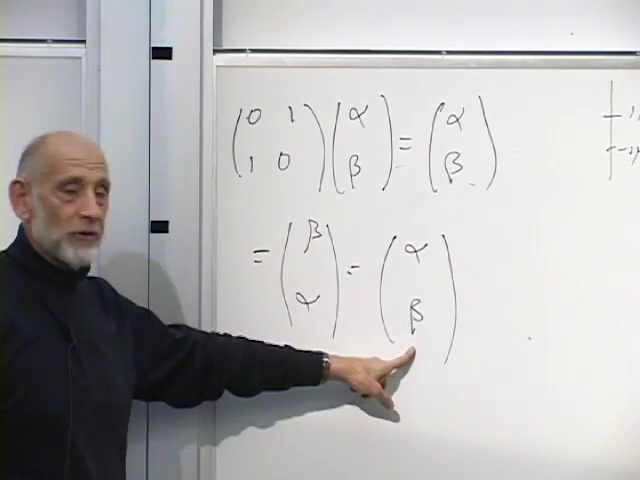
\includegraphics[width=0.74\textwidth]{lecture_08_figure_03.png}
\caption{Pour la valeur propre \(+1\), \(\sigma_x\) échange les deux composantes, ce qui impose \(\alpha=\beta\).}
\lectureframe{00:39:42}\end{figure}

\begin{classroomqa}\lecturetimestamp{00:40:13}\audiencequestion{Si le facteur un demi était inclus, la valeur propre serait-elle un demi ?}\lecturerresponse{Oui. La matrice de Pauli \(\sigma_x\) a pour valeurs propres \(\pm1\), tandis que \(S_x=\sigma_x/2\) a pour valeurs propres \(\pm\tfrac12\).}\end{classroomqa}

Pour la valeur propre \(-1\),
\begin{equation}
\begin{pmatrix}
\beta\\
\alpha
\end{pmatrix}
=
-
\begin{pmatrix}
\alpha\\
\beta
\end{pmatrix},
\end{equation}
donc
\begin{equation}
\beta=-\alpha,
\qquad
\alpha=-\beta.
\end{equation}
Ce sont à nouveau deux écritures de la même équation. Après normalisation,
\begin{equation}
|-x\rangle
=
\frac{1}{\sqrt2}
\begin{pmatrix}
1\\
-1
\end{pmatrix}.
\end{equation}
Ainsi, une superposition équipondérée des états de spin \(z\) positif et \(z\) négatif est polarisée selon l’axe \(x\) positif ; la même superposition avec un signe moins relatif est polarisée selon l’axe \(x\) négatif.

Dans la direction \(y\),
\begin{equation}
\sigma_y
\begin{pmatrix}
\alpha\\
\beta
\end{pmatrix}
=
\begin{pmatrix}
-i\beta\\
i\alpha
\end{pmatrix}.
\end{equation}
Les deux vecteurs propres normalisés sont
\begin{equation}
|+y\rangle
=
\frac{1}{\sqrt2}
\begin{pmatrix}
1\\
i
\end{pmatrix},
\qquad
|-y\rangle
=
\frac{1}{\sqrt2}
\begin{pmatrix}
1\\
-i
\end{pmatrix},
\end{equation}
à une phase globale près. Les deux états donnent une probabilité \(1/2\) d’obtenir un spin \(z\) positif et \(1/2\) d’obtenir un spin \(z\) négatif. La phase relative \(i\), invisible dans ces deux probabilités, distingue la polarisation selon \(y\) de celle selon \(x\). Les combinaisons linéaires décrivent aussi un spin polarisé selon des directions quelconques ; ce calcul est remis à plus tard.

\begin{classroomqa}\lecturetimestamp{00:44:22}\audiencequestion{Le signe de la composante \(i\) a-t-il été attribué à la mauvaise valeur propre de \(\sigma_y\) ?}\lecturerresponse{Le signe a effectivement pu être attribué à la mauvaise valeur propre. Cette attribution reste incertaine ici ; elle n’est pas fixée de mémoire.}\end{classroomqa}

Le calcul direct donne
\begin{align}
\sigma_y\frac{1}{\sqrt2}
\begin{pmatrix}
1\\
i
\end{pmatrix}
&=
\frac{1}{\sqrt2}
\begin{pmatrix}
-i\,i\\
i
\end{pmatrix}
=
\frac{1}{\sqrt2}
\begin{pmatrix}
1\\
i
\end{pmatrix},\\
\sigma_y\frac{1}{\sqrt2}
\begin{pmatrix}
1\\
-i
\end{pmatrix}
&=
\frac{1}{\sqrt2}
\begin{pmatrix}
(-i)(-i)\\
i
\end{pmatrix}
=
-\frac{1}{\sqrt2}
\begin{pmatrix}
1\\
-i
\end{pmatrix}.
\end{align}
Ainsi, \(+i\) correspond à la valeur propre \(+1\), et \(-i\) à la valeur propre \(-1\).\footnote{L’attribution orale reste indécise après plusieurs revirements ; les signes indiqués ici sont déterminés par le produit matriciel affiché.}Tout état de spin 1/2, y compris tout état polarisé selon une direction arbitraire, est une combinaison linéaire de \(|+z\rangle\) et de \(|-z\rangle\).

\section{Spin un et spineurs dépendant de la position}

Pour un spin \(1\), les valeurs possibles de \(S_z\) sont \(+1,0,-1\). L’espace d’états est donc de dimension trois. Le spin \(1\) est un spin entier et correspond à des statistiques bosoniques. Nous cherchons trois matrices \(3\times3\) satisfaisant aux mêmes relations de commutation du moment cinétique.

On trouvera ci-dessous une représentation symétrique par rapport aux trois directions de coordonnées.\footnote{Le signe de \(S_y\) découle de la matrice visible vers \(00{:}48{:}50\) et est également déterminé par \([S_x,S_y]=iS_z\). L’inverser inverserait le signe du commutateur requis.}
\begin{equation}
\begin{aligned}
S_x
&=
i
\begin{pmatrix}
0&0&0\\
0&0&1\\
0&-1&0
\end{pmatrix},
&
S_y
&=
i
\begin{pmatrix}
0&0&1\\
0&0&0\\
-1&0&0
\end{pmatrix},\\
S_z
&=
i
\begin{pmatrix}
0&1&0\\
-1&0&0\\
0&0&0
\end{pmatrix}.
\end{aligned}
\end{equation}
Chaque matrice est égale à \(i\) fois une matrice réelle antisymétrique. Chacune contient un \(1\), un \(-1\), et une ligne ainsi qu’une colonne nulles associées à sa propre coordonnée : la première pour \(S_x\), la deuxième pour \(S_y\) et la troisième pour \(S_z\). Cela fournit un moyen mnémotechnique utile. Dans cette représentation, \(S_z\) n’est pas diagonale.

Posons
\begin{equation}
v=
\begin{pmatrix}
\alpha\\
\beta\\
\gamma
\end{pmatrix}.
\end{equation}
Alors
\begin{equation}
S_zv
=
\begin{pmatrix}
i\beta\\
-i\alpha\\
0
\end{pmatrix}.
\end{equation}
Pour la valeur propre \(+1\),
\begin{equation}
i\beta=\alpha,
\qquad
-i\alpha=\beta,
\qquad
0=\gamma.
\end{equation}
On a donc \(\beta=-i\alpha\) et \(\gamma=0\). La normalisation impose \(2|\alpha|^2=1\), d’où
\begin{equation}
|m=+1\rangle
=
\frac{1}{\sqrt2}
\begin{pmatrix}
1\\
-i\\
0
\end{pmatrix}.
\end{equation}
Pour la valeur propre \(-1\),
\begin{equation}
i\beta=-\alpha,
\qquad
-i\alpha=-\beta,
\qquad
0=-\gamma,
\end{equation}
d’où \(\beta=i\alpha\), \(\gamma=0\) et
\begin{equation}
|m=-1\rangle
=
\frac{1}{\sqrt2}
\begin{pmatrix}
1\\
i\\
0
\end{pmatrix}.
\end{equation}
Enfin, l’équation associée à la valeur propre nulle donne \(\alpha=\beta=0\), tandis que \(\gamma\) reste arbitraire. Sa solution normalisée est
\begin{equation}
|m=0\rangle
=
\begin{pmatrix}
0\\
0\\
1
\end{pmatrix}.
\end{equation}
Il n’y a pas d’autres valeurs propres : ces trois vecteurs propres engendrent tout l’espace de dimension trois. Les facteurs \(1/\sqrt2\) ne sont pas de simples ornements. Ces mêmes coefficients interviendront plus tard dans les prédictions expérimentales quantitatives, lorsque l’algèbre sera appliquée à l’isospin.

\begin{classroomqa}\lecturetimestamp{00:54:10}\audiencequestion{Comment faut-il lire les composantes complexes de ces vecteurs propres de spin un ?}\lecturerresponse{Pour \(m=+1\), les composantes sont \(1/\sqrt2,-i/\sqrt2,0\) ; pour \(m=-1\), elles sont \(1/\sqrt2,i/\sqrt2,0\) ; et pour \(m=0\), elles sont \(0,0,1\).}\end{classroomqa}

D’autres triplets de matrices satisfont à la même algèbre et sont physiquement équivalents. La représentation symétrique ci-dessus est utile parce qu’elle traite les trois directions de la même façon ; nous la réutiliserons.

\subsection{Rétablir la position}

Rétablissons maintenant le mouvement de la particule. Le spin commute avec la position et avec l’impulsion ; l’une ou l’autre peut donc être spécifiée conjointement à une composante du spin. La position et l’impulsion ne commutent pas, et les différentes composantes du spin ne commutent pas non plus entre elles.

Une particule de spin un demi en mouvement est décrite par un spineur dépendant de la position,
\begin{equation}
\psi(x)=
\begin{pmatrix}
\psi_\uparrow(x)\\
\psi_\downarrow(x)
\end{pmatrix}.
\end{equation}
Les grandeurs
\begin{equation}
\rho_{\uparrow_z}(x)=|\psi_\uparrow(x)|^2,
\qquad
\rho_{\downarrow_z}(x)=|\psi_\downarrow(x)|^2
\end{equation}
sont des densités de probabilité conjointes de position et de spin. Leur somme,
\begin{equation}
\rho(x)=\psi^\dagger(x)\psi(x)
=|\psi_\uparrow(x)|^2+|\psi_\downarrow(x)|^2,
\end{equation}
est la densité de position. Si l’on sait que la particule a été détectée en \(x\), les probabilités conditionnelles sont
\begin{equation}
P(\uparrow_z\mid x)
=
\frac{|\psi_\uparrow(x)|^2}{\psi^\dagger(x)\psi(x)},
\qquad
P(\downarrow_z\mid x)
=
\frac{|\psi_\downarrow(x)|^2}{\psi^\dagger(x)\psi(x)},
\end{equation}
lorsque \(\rho(x)\neq0\). Un électron est donc représenté par une fonction d’onde spatiale à deux composantes, dont les amplitudes locales de spin peuvent varier d’un point à l’autre.

Pour une particule de spin un en mouvement, écrivons
\begin{equation}
\phi(x)=
\begin{pmatrix}
\phi_1(x)\\
\phi_2(x)\\
\phi_3(x)
\end{pmatrix}.
\end{equation}
En chaque point de l’espace, les trois composantes forment un vecteur dans le même espace de spin que précédemment. Les particules de spin un ont un spin entier et sont des bosons.

\begin{classroomqa}\lecturetimestamp{01:00:10}\audiencequestion{\(\phi_1(x)\) est-elle à elle seule la probabilité d’obtenir la valeur \(m=+1\) pour le spin un ?}\lecturerresponse{Non. C’est une amplitude dans la base à trois composantes choisie. Pour obtenir une valeur déterminée du spin, il faut former le bra du vecteur propre normalisé correspondant, projeter le champ sur celui-ci et prendre le carré du module.}\end{classroomqa}

\begin{figure}[t]
\centering
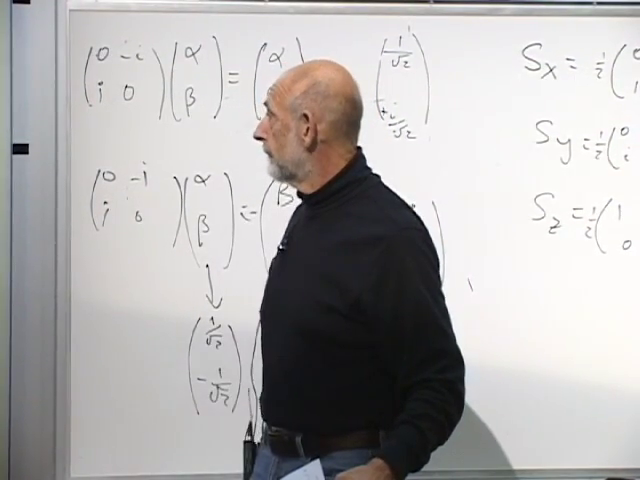
\includegraphics[width=0.82\textwidth]{lecture_08_figure_04.png}
\caption{Vecteurs propres normalisés de \(\sigma_y\) à côté des trois matrices de spin un demi.}
\lectureframe{01:00:12}\end{figure}

Par exemple,
\begin{equation}
\begin{aligned}
|m=+1\rangle
&=
\frac{1}{\sqrt2}
\begin{pmatrix}
1\\
-i\\
0
\end{pmatrix}
\\
\Longrightarrow\quad\langle m=+1|
&=
\frac{1}{\sqrt2}
\begin{pmatrix}
1&i&0
\end{pmatrix}.
\end{aligned}
\end{equation}
L’amplitude de projection est donc
\begin{align}
\langle m=+1|\phi(x)\rangle
&=
\frac{1}{\sqrt2}
\begin{pmatrix}
1&i&0
\end{pmatrix}
\begin{pmatrix}
\phi_1(x)\\
\phi_2(x)\\
\phi_3(x)
\end{pmatrix}\\
&=
\frac{\phi_1(x)+i\phi_2(x)}{\sqrt2}.
\end{align}
La même règle appliquée aux trois vecteurs propres donne les densités résolues en spin.\footnote{Ces formules achèvent l’algèbre de projection après la correction explicite : \(\phi_1\) et \(\phi_2\) ne sont pas nécessairement réelles. Les traiter comme des quantités réelles effacerait à tort l’interférence qui distingue les densités \(m=+1\) et \(m=-1\).}
\begin{align}
\rho_{+1}(x)
&=
\frac12\left|\phi_1(x)+i\phi_2(x)\right|^2,\\
\rho_{-1}(x)
&=
\frac12\left|\phi_1(x)-i\phi_2(x)\right|^2,\\
\rho_0(x)
&=
|\phi_3(x)|^2.
\end{align}
Elles vérifient
\begin{equation}
\begin{aligned}
\rho_{+1}(x)+\rho_{-1}(x)+\rho_0(x)
&=
|\phi_1(x)|^2+|\phi_2(x)|^2
\\
&\quad{}+|\phi_3(x)|^2
\\
&=
\phi^\dagger(x)\phi(x).
\end{aligned}
\end{equation}
Si la détection de la particule est conditionnée à sa présence en \(x\), alors
\begin{equation}
P(m\mid x)
=
\frac{\rho_m(x)}{\phi^\dagger(x)\phi(x)},
\end{equation}
à condition que \(\phi^\dagger(x)\phi(x)\neq0\). La règle générale de mesure est toujours la même : former le bra du vecteur propre normalisé recherché, projeter l’état réel sur celui-ci, puis prendre le carré du module. La densité obtenue conserve sa dépendance en position.

Les matrices de spin supérieur sont plus compliquées, mais le principe reste le même.

\begin{classroomqa}\lecturetimestamp{01:07:31}\audiencequestion{Quelle est la dimension de l’espace d’états pour le spin trois demis ?}\lecturerresponse{Il comporte quatre états, avec \(m=\tfrac32,\tfrac12,-\tfrac12,-\tfrac32\). Le spin deux en comporte cinq.}\end{classroomqa}

\begin{classroomqa}\lecturetimestamp{01:07:55}\audiencequestion{Pourquoi la discussion a-t-elle fait intervenir \(x,y,z\) sans direction temporelle ? Ce traitement est-il non relativiste ?}\lecturerresponse{Jusqu’ici, le traitement est non relativiste. Le spin, comme la masse, se caractérise le plus simplement dans le référentiel de repos de la particule ; sa description dans un autre référentiel inertiel s’obtient par la transformation de Lorentz appropriée. Cette étape relativiste est remise à plus tard.}\end{classroomqa}

L’équation de Dirac fournit le cadre relativiste et explique pourquoi sa fonction d’onde à quatre composantes contient un doublet de spin.

\section{Matrices de Dirac et spineur à quatre composantes}

La fonction d’onde de Dirac à quatre composantes vérifie
\begin{equation}
i\frac{\partial\Psi}{\partial t}
=
-i\alpha_i\frac{\partial\Psi}{\partial x_i}
+m\beta\Psi,
\qquad i=1,2,3,
\end{equation}
où tout indice spatial répété est sommé. Le terme dérivé signifie donc
\begin{equation}
\alpha_1\frac{\partial\Psi}{\partial x}
+\alpha_2\frac{\partial\Psi}{\partial y}
+\alpha_3\frac{\partial\Psi}{\partial z}.
\end{equation}
Pour une onde plane, l’équation devient l’équation algébrique
\begin{equation}
\omega\Psi=(\alpha_i k_i+m\beta)\Psi.
\end{equation}

\begin{classroomqa}\lecturetimestamp{01:11:32}\audiencequestion{Les deux occurrences de \(m\) désignent-elles la même chose ?}\lecturerresponse{Non. L’une servait d’indice spatial, tandis que l’autre désigne la masse de la particule. Renommons l’indice spatial \(i\) ; lorsque \(i\) apparaît deux fois, on somme cet indice de \(1\) à \(3\).}\end{classroomqa}

Le carré de l’opérateur fréquence doit redonner la relation relativiste
\begin{equation}
\omega^2=\mathbf{k}^2+m^2.
\end{equation}
Les termes carrés imposent donc, pour chaque \(i\),
\begin{equation}
\alpha_i^2=I_4,
\qquad
\beta^2=I_4.
\end{equation}

\begin{classroomqa}\lecturetimestamp{01:13:01}\audiencequestion{\(\beta\) est-elle différente pour chacune des quatre composantes de \(\Psi\) ?}\lecturerresponse{Non. Il n’y a qu’une matrice \(\beta\), qui agit sur le spineur à quatre composantes entier et vérifie \(\beta^2=I_4\).}\end{classroomqa}

Les termes croisés doivent s’annuler. Pour des directions spatiales différentes, et aussi entre chaque \(\alpha_i\) et \(\beta\), on obtient
\begin{equation}
\alpha_i\alpha_j+\alpha_j\alpha_i=0
\quad (i\neq j),
\qquad
\alpha_i\beta+\beta\alpha_i=0.
\end{equation}
De manière équivalente,
\begin{equation}
\{\alpha_i,\alpha_j\}=2\delta_{ij}I_4,
\quad
\{\alpha_i,\beta\}=0,
\quad
\{\beta,\beta\}=2I_4.
\end{equation}
Chaque matrice anticommmute avec toute matrice différente, tandis que son anticommutateur avec elle-même est égal à deux fois l’identité.

Sans \(\beta\), les trois matrices de Pauli fourniraient déjà trois matrices \(2\times2\) dont le carré est l’identité et qui anticommutent deux à deux. Le terme de masse exige une quatrième matrice de ce type. Il n’existe pas de quatrième matrice \(2\times2\) possédant les propriétés requises, et les matrices \(3\times3\) ne satisfont pas non plus à l’algèbre. La représentation de plus petite dimension est donc \(4\times4\).

Une matrice \(4\times4\) peut être divisée en quatre blocs \(2\times2\). Dans une représentation commode,
\begin{equation}
\alpha_i=
\begin{pmatrix}
\sigma_i&0\\
0&-\sigma_i
\end{pmatrix},
\qquad i=1,2,3.
\end{equation}

\begin{figure}[t]
\centering
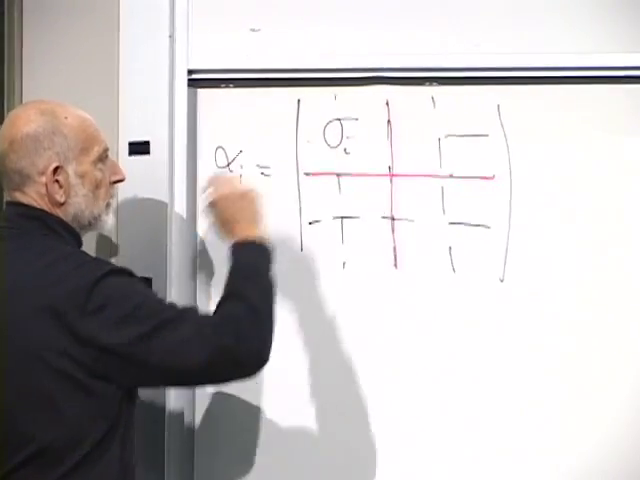
\includegraphics[width=0.68\textwidth]{lecture_08_figure_05.png}
\caption{La matrice de Dirac \(\alpha_i\) écrite en blocs \(2\times2\), avec \(\sigma_i\) et \(-\sigma_i\) sur la diagonale.}
\lectureframe{01:17:23}\end{figure}

\begin{classroomqa}\lecturetimestamp{01:17:41}\audiencequestion{Les blocs \(\sigma_i\) étaient-ils disposés autrement dans la représentation précédente ?}\lecturerresponse{Oui. Dans une autre représentation, ils étaient placés hors de la diagonale. Les deux dispositions sont équivalentes et reliées par une transformation de similitude.}\end{classroomqa}

Dans la représentation actuelle, la matrice restante est
\begin{equation}
\beta=
\begin{pmatrix}
0&I_2\\
I_2&0
\end{pmatrix},
\qquad
I_2=
\begin{pmatrix}
1&0\\
0&1
\end{pmatrix}.
\end{equation}
La multiplication par blocs ramène la vérification de l’algèbre \(4\times4\) à des multiplications ordinaires de matrices \(2\times2\).

\begin{classroomqa}\lecturetimestamp{01:19:17}\audiencequestion{La représentation précédente utilisait-elle un signe différent ou une forme diagonale pour \(\beta\) ?}\lecturerresponse{Elle utilisait une base différente, mais physiquement équivalente. Un changement de base mélange les quatre composantes de \(\Psi\) et modifie l’apparence des matrices sans changer la physique.}\end{classroomqa}

Les quatre composantes de \(\Psi\) ne sont pas les quatre coordonnées de l’espace-temps. Ce sont des coordonnées dans le plus petit espace vectoriel sur lequel cette algèbre d’anticommutation peut agir. Il y a deux structures distinctes de dimension deux : la décomposition en blocs \(2\times2\) et la structure de Pauli à deux composantes à l’intérieur de chaque bloc. En anticipant l’interprétation qui sera établie ci-dessous, on peut organiser les quatre possibilités comme suit :
\begin{equation}
\begin{array}{c|cc}
& S_z=+\tfrac12 & S_z=-\tfrac12\\ \hline
\omega>0 & (\omega>0,+\tfrac12) & (\omega>0,-\tfrac12)\\
\omega<0 & (\omega<0,+\tfrac12) & (\omega<0,-\tfrac12)
\end{array}.
\end{equation}
La ligne du bas correspond aux états électroniques de fréquence négative. Ce n’est pas une ligne de positrons ; un positron sera interprété comme un trou dans l’ensemble rempli de ces états.

\section{Doublement de l’énergie au repos et positron}

La structure de doublement de l’énergie apparaît le plus clairement à impulsion nulle. Lorsque \(\mathbf{k}=0\), l’état d’onde plane est spatialement constant et le terme de dérivée spatiale disparaît. L’équation dans le référentiel de repos\footnote{La séquence à \(01{:}23{:}38\) conserve temporairement un facteur supplémentaire \(i\) devant le terme de masse ; la correction orale à \(01{:}24{:}05\) le supprime.}est
\begin{equation}
i\frac{\partial\Psi}{\partial t}=m\beta\Psi.
\end{equation}

\begin{figure}[t]
\centering
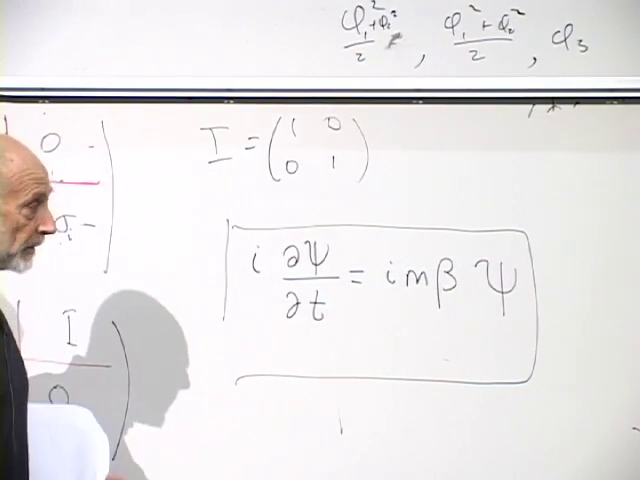
\includegraphics[width=0.76\textwidth]{lecture_08_figure_06.png}
\caption{À impulsion nulle, les dérivées spatiales s’annulent, ce qui laisse l’équation corrigée dans le référentiel de repos \(i\partial_t\Psi=m\beta\Psi\).}
\lectureframe{01:23:38}\end{figure}

Divisons la colonne à quatre composantes en un objet à deux composantes supérieur et un autre inférieur :
\begin{equation}
\Psi=
\begin{pmatrix}
\psi_+\\
\psi_-
\end{pmatrix}.
\end{equation}

\begin{classroomqa}
\lecturetimestamp{01:24:47}
\audiencequestion{Les étiquettes \(\psi_+\) et \(\psi_-\) désignent-elles déjà les énergies positive et négative ?}
\lecturerresponse{Non. À ce stade, ce ne sont que des noms pour les blocs supérieur et inférieur à deux composantes. Les combinaisons correspondant à leurs énergies n’ont pas encore été déterminées.}
\end{classroomqa}

\begin{classroomqa}
\lecturetimestamp{01:25:10}
\audiencequestion{Que représente la colonne à quatre composantes décomposée ?}
\lecturerresponse{C’est le même spineur de Dirac à quatre composantes, organisé de façon à correspondre à la forme par blocs des matrices. Chaque moitié est un objet à deux composantes, et ces deux objets forment la colonne initiale à quatre composantes.}
\end{classroomqa}

La matrice \(\beta\) échange les deux blocs :
\begin{equation}
\beta
\begin{pmatrix}
\psi_+\\
\psi_-
\end{pmatrix}
=
\begin{pmatrix}
\psi_-\\
\psi_+
\end{pmatrix}.
\end{equation}
L’équation au repos devient donc
\begin{equation}
i\frac{\partial\psi_+}{\partial t}=m\psi_-,
\qquad
i\frac{\partial\psi_-}{\partial t}=m\psi_+.
\end{equation}

Deux possibilités s’imposent naturellement. Prendre une dérivée temporelle supplémentaire découplerait le système, mais la somme et la différence des deux équations le diagonalisent immédiatement. En effet,
\begin{align}
i\frac{\partial}{\partial t}(\psi_++\psi_-)
&=m(\psi_++\psi_-),\\
i\frac{\partial}{\partial t}(\psi_+-\psi_-)
&=-m(\psi_+-\psi_-).
\end{align}
En posant
\begin{equation}
\chi_+=\psi_++\psi_-,
\qquad
\chi_-=\psi_+-\psi_-,
\end{equation}
on obtient deux équations indépendantes :
\begin{equation}
i\partial_t\chi_+=m\chi_+,
\qquad
i\partial_t\chi_-=-m\chi_-.
\end{equation}
Pour une dépendance temporelle de fréquence définie \(e^{-i\omega t}\), la somme vérifie
\begin{equation}
\omega=+m,
\end{equation}
tandis que la différence vérifie
\begin{equation}
\omega=-m.
\end{equation}
On retrouve exactement le dédoublement en énergies positive et négative de l’exemple unidimensionnel étudié précédemment : l’équation relativiste admet, elle aussi, des solutions électroniques d’énergie positive et d’énergie négative. Le dédoublement des blocs se sépare donc en branches d’énergie positive et négative. Les états purs au repos peuvent s’écrire
\begin{equation}
\Psi_{\omega=+m}=
\begin{pmatrix}
\xi\\
\xi
\end{pmatrix},
\qquad
\Psi_{\omega=-m}=
\begin{pmatrix}
\xi\\
-\xi
\end{pmatrix},
\end{equation}
où \(\xi\) reste un objet arbitraire à deux composantes.

La somme et la différence ont éliminé une structure à deux états, mais les deux composantes de \(\xi\) subsistent. Les matrices de Pauli agissent sur cette paire résiduelle. Il s’agit de la paire associée au spin, sous réserve de vérifier les transformations par rotation et les lois de conservation, comme on le verra plus loin.

\begin{classroomqa}
\lecturetimestamp{01:32:23}
\audiencequestion{Peut-on considérer le spin comme la structure extérieure à deux états et le signe de l’énergie comme la structure intérieure ?}
\lecturerresponse{Oui. Les deux ordres des facteurs sont équivalents. On peut échanger l’indice écrit en premier ; cela ne fait que réarranger les quatre composantes.}
\end{classroomqa}

La branche de fréquence négative conduit à l’interprétation de la mer de Dirac. Une fréquence négative est associée à une énergie électronique négative. Remplir tous les états électroniques d’énergie négative abaisse l’énergie autant que le permet le principe d’exclusion, puisque chaque état fermionique complet ne peut être occupé que par un seul électron. La mer d’énergie négative ainsi entièrement remplie est alors appelée le vide.

Promouvons un électron de cette mer remplie vers un état d’énergie positive. On obtient alors un électron d’énergie positive et un état d’énergie négative inoccupé. Retirer une énergie négative augmente l’énergie ; le trou possède donc une énergie d’excitation positive. Comme il correspond à un électron manquant, il porte aussi la charge électrique opposée. Ce trou est un positron.

\begin{classroomqa}
\lecturetimestamp{01:32:57}
\audiencequestion{Pouvez-vous expliquer encore une fois l’interprétation du positron ?}
\lecturerresponse{La somme des deux blocs est de fréquence positive et leur différence, de fréquence négative. Les solutions de fréquence négative sont des états électroniques d’énergie négative, et le vide s’obtient en les remplissant tous. Promouvoir un électron de la mer remplie vers une énergie positive laisse à la fois un électron d’énergie positive et un trou. Ce trou d’énergie positive et de charge opposée est le positron.}
\end{classroomqa}

L’algèbre a donc produit simultanément deux conséquences : des branches d’énergie positive et négative, qui donnent la structure particule--antiparticule, et une structure résiduelle à deux composantes associée au spin un demi. Le fait remarquable est que toutes deux sont issues des plus petites matrices capables de satisfaire les relations d’anticommutation relativistes. Le spin venait tout juste d’apparaître comme propriété empirique lorsque cette construction mathématique a fait surgir des particules dotées d’un spin ainsi qu’une branche d’antiparticule ; dans ce contexte historique, le résultat était spectaculaire.

\begin{classroomqa}
\lecturetimestamp{01:35:14}
\audiencequestion{Les électrons d’énergie négative sont-ils eux-mêmes des positrons ?}
\lecturerresponse{Non. Les états électroniques d’énergie négative sont remplis dans le vide. Un positron est l’absence d’un électron dans cet ensemble rempli : c’est un trou, et non un électron d’énergie négative.}
\end{classroomqa}

Un trou peut participer à des transitions. Un positron possède une énergie positive parce qu’il correspond à l’absence d’un électron d’énergie négative. Si un électron d’énergie positive comble le trou, l’électron et le positron s’annihilent, mais leur énergie doit être emportée, ordinairement par des photons. Dans le langage de la mer, un électron a occupé un état d’énergie négative inoccupé. On peut représenter la même libération d’énergie par un électron excité dans un atome qui descend vers un niveau inférieur : cette transition descendante émet des photons.

\begin{classroomqa}
\lecturetimestamp{01:36:39}
\audiencequestion{Pourquoi les électrons d’énergie négative situés à des niveaux supérieurs ne tombent-ils pas dans le trou ?}
\lecturerresponse{Cette question confond deux cas. Lorsqu’un électron d’énergie positive comble le trou, il s’agit d’une annihilation électron--positron, l’énergie étant emportée par des photons. Une transition impliquant un électron de la mer d’énergie négative est un processus différent, qui sera abordé plus loin.}
\end{classroomqa}

Le calcul à impulsion nulle établit à lui seul une dégénérescence double une fois le signe de l’énergie séparé. Une dégénérescence entre deux états ne prouve pas, à elle seule, que ces états portent un moment cinétique.

\begin{classroomqa}
\lecturetimestamp{01:37:44}
\audiencequestion{Comment le calcul à impulsion nulle prouve-t-il que la paire d’états restante correspond au spin ?}
\lecturerresponse{On peut appeler les états « spin haut » et « spin bas », et les matrices de Pauli apparaissent dans l’équation complète, mais cela ne constitue pas encore une preuve. Il faut montrer soit comment la paire se transforme sous l’effet des rotations spatiales, soit que lui attribuer un spin rend le moment cinétique total conservé lors des interactions et des collisions. Cette démonstration est reportée à plus tard.}
\end{classroomqa}

Pour un état au repos d’énergie positive, les blocs supérieur et inférieur sont égaux :
\begin{equation}
\Psi_{\omega=+m}=
\begin{pmatrix}
\xi\\
\xi
\end{pmatrix}.
\end{equation}
Établir que \(\xi\) forme un doublet de moment cinétique exige l’argument fondé sur les rotations ou la conservation évoqué plus haut ; cela ne découle pas du simple décompte des deux composantes.

\begin{classroomqa}
\lecturetimestamp{01:40:46}
\audiencequestion{Un autre électron peut-il s’annihiler avec le positron même si son énergie est différente ?}
\lecturerresponse{Oui. Les électrons ne conservent aucune identité individuelle. L’un ou l’autre des électrons disponibles peut combler le trou ; les différences d’énergie et d’impulsion initiales se reflètent dans le nombre et les énergies des photons émis.}
\end{classroomqa}

L’image du trou explique aussi une transition qui se produit entièrement au sein de la mer d’énergie négative. Supposons qu’un état occupé d’énergie négative passe dans le trou. Le trou initial est comblé, mais l’état d’où provenait cet électron est désormais vide. Le trou s’est déplacé. De manière équivalente, le positron a changé d’énergie et a émis un rayonnement.

\begin{classroomqa}
\lecturetimestamp{01:42:12}
\audiencequestion{Pourquoi les niveaux d’énergie négative voisins ne peuvent-ils pas tomber successivement dans le trou ?}
\lecturerresponse{Ils peuvent déplacer le trou d’un niveau à un autre. Un électron qui tombe dans l’ancien trou laisse un nouveau trou à l’énergie qu’il occupait auparavant ; le positron initial devient donc un positron d’énergie différente. La différence d’énergie est emportée par des photons.}
\end{classroomqa}

\begin{classroomqa}
\lecturetimestamp{01:44:39}
\audiencequestion{Pourquoi cela ne provoque-t-il pas une cascade radiative descendante sans fin ?}
\lecturerresponse{Parce que l’énergie et l’impulsion doivent être conservées simultanément. Ces deux lois de conservation ne permettent pas un processus sans restriction. Le même problème se pose pour un électron libre ordinaire : il ne peut pas continuer simplement à abaisser son énergie en émettant des photons dans le vide.}
\end{classroomqa}
